\documentclass[11pt]{article}
\usepackage[margin=0.7in]{geometry}
\usepackage{amsmath,amssymb}
\usepackage{enumitem}
\usepackage{tikz}
\usepackage{pgfplots}
\pgfplotsset{compat=1.18}
\usepackage{fancyhdr}
\usepackage{parskip}
\setlist[enumerate]{leftmargin=*, itemsep=6pt}
\pagestyle{fancy}
\fancyhf{}
\fancyfoot[L]{\small\textit{en}Vision\textsuperscript{\textregistered} Algebra 2}
\fancyfoot[C]{\small 3-2 Lesson Quiz, short form}
\fancyfoot[R]{\small\thepage}
\renewcommand{\headrulewidth}{0pt}
\newcommand{\choice}[1]{\tikz[baseline=-0.6ex]\node[draw, circle, inner sep=0.6pt, minimum size=3.3mm, font=\scriptsize\bfseries] {#1};\;}
\newcommand{\tile}[1]{\tikz[baseline=-0.6ex]\node[draw, rounded corners=2pt, minimum height=6.5mm, minimum width=12mm, inner sep=2pt] {$#1$};}
\newcommand{\ansbox}{\tikz[baseline=-0.6ex]\node[draw, minimum height=8mm, minimum width=22mm] {};}

\begin{document}

\noindent\textbf{Name}\; \rule{6cm}{0.4pt} \hfill Period \rule{1.2cm}{0.4pt} \quad Date \rule{2.2cm}{0.4pt}

\vspace{4pt}\noindent\rule{\textwidth}{0.6pt}

\vspace{2pt}\noindent{\Large\textbf{3-2 \; Lesson Quiz: Adding, Subtracting, and Multiplying Polynomials}}

\noindent{\small short form \hfill questions keep their Savvas numbers (1, 2, 4); show your work}

\vspace{2pt}\noindent\rule{\textwidth}{0.6pt}

\vspace{6pt}
\textbf{1.} Add $(4a^2b-3ab^2+2ab+5)$ and $(2a^2b+3ab^2-7ab)$. Complete the expression in standard form. Write one tile in each box.

\vspace{4pt}
\begin{center}
\tile{a^2b}\; \tile{6a^2b}\; \tile{6ab^2}\; \tile{(-9ab^2)}\; \tile{(-5ab)}\; \tile{9ab}\; \tile{5ab}\; \tile{5}
\end{center}

\vspace{2pt}
\begin{center}
\ansbox \;\; $+$ \;\; \ansbox \;\; $+$ \;\; \ansbox
\end{center}

Work:

\vspace{1.3cm}

\noindent\rule{\textwidth}{0.4pt}

\vspace{6pt}
\textbf{2.} Multiply $(x+2y)(x^2-xy+3y)$.

\vspace{4pt}
\begin{itemize}[leftmargin=1.2em, itemsep=5pt]
\item[] \choice{A} $x^3+x^2y+3xy-2xy^2+6y^2$
\item[] \choice{B} $x^3-3x^2y+3xy-2xy^2+6y^2$
\item[] \choice{C} $x^3+3xy-xy^2+3y^2$
\item[] \choice{D} $x^3-xy+6y^2$
\end{itemize}

Work:

\vspace{1.8cm}

\noindent\rule{\textwidth}{0.4pt}

\vspace{6pt}
\begin{minipage}[t]{0.62\textwidth}
\textbf{4.} Jae is constructing an open box from a piece of cardboard that is 9 in. wide and 12 in. long. Jae cuts squares of equal size from each corner of the cardboard, and then folds up the sides of the box. Write and simplify a polynomial function $V$ in standard form for the volume of the box in terms of $x$.

\vspace{8pt}
$V(x)=\rule{1.4cm}{0.4pt}\,x^3-\rule{1.4cm}{0.4pt}\,x^2+\rule{1.4cm}{0.4pt}\,x$

\vspace{4pt}
Work:
\end{minipage}\hfill
\begin{minipage}[t]{0.34\textwidth}
\vspace{0pt}
\begin{center}
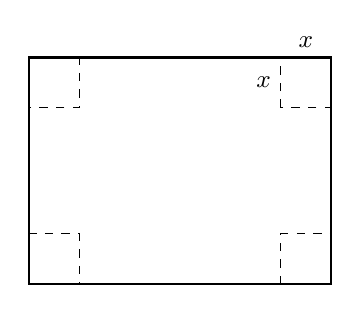
\begin{tikzpicture}[scale=0.32]
\draw[thick] (0,0) rectangle (12,9);
\foreach \a/\b in {0/0, 10/0, 0/7, 10/7} {\draw[dashed] (\a,\b) rectangle ++(2,2);}
\node[above, font=\small] at (11,9) {$x$};
\node[left, font=\small] at (10,8) {$x$};
\end{tikzpicture}
\end{center}
\end{minipage}

\vfill
\noindent\textbf{Scoring:} Question 2 and Question 4 are 10 points each. Question 1 is a bonus of up to 5 points. Total out of 20.

\newpage
\noindent{\LARGE\textbf{3-2 Lesson Quiz, short form: answer key}}

\vspace{4pt}\noindent\rule{\textwidth}{0.6pt}

\begin{enumerate}
\item[\textbf{1.}] \textbf{$6a^2b+(-5ab)+5$.} Like terms: $4a^2b+2a^2b=6a^2b$; $-3ab^2+3ab^2=0$ (the $ab^2$ terms cancel, so no $ab^2$ tile is used); $2ab-7ab=-5ab$; the constant is $5$. Standard form: degree 3, then degree 2, then the constant. Savvas quiz item 1, DOK 1, Skills Review and Practice A18 (IXL 9A3). Example 1 teaches it and is skipped in the fast packet; the 9A3 Jam and the subtraction step in Example 4 (distribute $-1$, combine like terms) carry it. \textbf{Bonus 5:} 1 per correct box in the correct order (3), 2 for shown grouping of like terms.
\item[\textbf{2.}] \textbf{A, $x^3+x^2y+3xy-2xy^2+6y^2$.} $x(x^2-xy+3y)+2y(x^2-xy+3y)=x^3-x^2y+3xy+2x^2y-2xy^2+6y^2$, and $-x^2y+2x^2y=x^2y$. Choice B subtracts $2x^2y$ instead of adding it ($-3x^2y$); C and D leave out the $x^2y$ term and do not show all six products. Savvas quiz item 2, DOK 1, A20 (IXL 8GN). Taught by Example 2A. \textbf{10 points:} 6 for A, 4 for work that shows all six products.
\item[\textbf{4.}] \textbf{$V(x)=4x^3-42x^2+108x$.} Length $12-2x$, width $9-2x$, height $x$: $V(x)=x(12-2x)(9-2x)=x(108-24x-18x+4x^2)=x(4x^2-42x+108)$. Savvas quiz item 4, DOK 3, A20 (IXL 8GN). Taught by Example 4 (write a polynomial function from a situation), Example 2B (three factors, two first) and the packet Practice (TE Practice 27, the foundry tray, filed under Example 4 in the TE item analysis). \textbf{10 points:} 3 for the three dimensions (1 each), 1 for the product $x(12-2x)(9-2x)$, 6 for the simplified standard form (2 per coefficient).
\end{enumerate}

\textbf{Items left off this form} (available for a retake or Form B): Savvas item 3, closure of monomials under multiplication (answer C, ``Yes; the product of any two monomials is a monomial''; DOK 2, A20; it is Try It 3 of the cut Example 3); Savvas item 5, hemisphere $V(x)=\tfrac23\pi x^3$ versus the graphed cube volume over $[2,3]$ (answer: the hemisphere is increasing faster; DOK 2, F61; average rate of change, the cut Example 5 and Lesson 3-1). Item 5's graph ($y=x^3$, window $0\le x\le5$, $0\le y\le100$) could be redrawn; it is left off because no kept Example teaches it, not because of the figure.

\textbf{IXL replacement:} SmartScore 70 or above on 8GN and 9A3 (the starred skills) replaces this quiz with 20/20.

\end{document}
